

\section{Introduction}

\begin{frame}
		\frametitle{Problem Size/Compute Time Correlation}
			\begin{figure}
					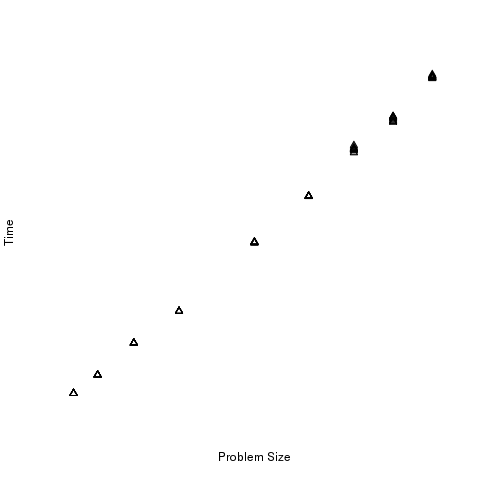
\includegraphics[width=0.65\linewidth]{figures/time/linpack}
			\end{figure}
\end{frame}

\begin{frame}
		\frametitle{Problem Size/Compute Time Correlation}
		laplace compute time
\end{frame}

\begin{frame}
		\frametitle{Problem Size/Memory Correlation}
			\begin{figure}
					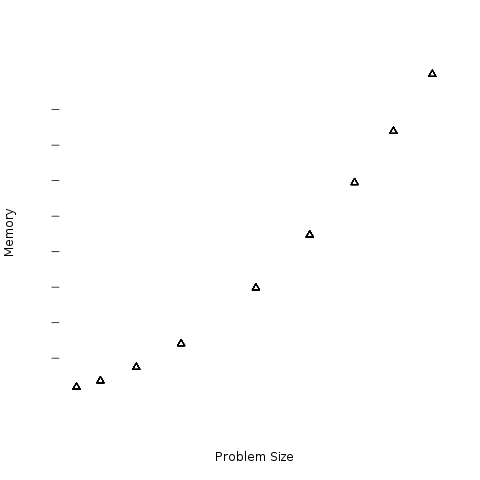
\includegraphics[width=0.65\linewidth]{figures/memory/linpack}
			\end{figure}
\end{frame}

\begin{frame}
		\frametitle{Problem Size/Memory Correlation}
		laplace memory usage
\end{frame}

\begin{frame}
		\frametitle{Combinations}
		\begin{itemize}
				\item Compute time increases only
				\item Memory usage increases only
				\item Compute time and Memory increases
		\end{itemize}
\end{frame}
